% =============================================
% CAPÍTULO 4 - GESTÃO DO PROJETO
% =============================================
\chapter{GESTÃO DO PROJETO}

A gestão do projeto é fundamental para garantir que o desenvolvimento da solução ocorra de forma organizada, controlada e alinhada aos objetivos estabelecidos. De acordo com a Enap, o gerenciamento de projetos consiste na aplicação de conhecimentos, habilidades, ferramentas e técnicas às atividades do projeto, envolvendo planejamento, execução e controle para atender aos requisitos definidos. Destaca-se que projetos são temporários e voltados à entrega de resultados únicos (ENAP, 2014), o que se aplica a este trabalho, já que o sistema proposto possui escopo, prazo e entregas previamente definidos.

Para apoiar essa organização, serão utilizadas ferramentas digitais que auxiliem a comunicação, o acompanhamento das tarefas e o desenvolvimento do sistema. O Trello será empregado na visualização e controle das atividades, enquanto o GitHub será utilizado para armazenamento e versionamento do código-fonte, favorecendo a colaboração entre os integrantes da equipe.

\section{Gerenciamento do projeto}

Para o gerenciamento do projeto, optou-se pela utilização de práticas ágeis, com destaque para o \textit{framework} Scrum, por sua flexibilidade e adequação ao desenvolvimento incremental de \textit{software}. Segundo o Guia do Scrum, essa abordagem permite organizar o trabalho em ciclos curtos, com entregas contínuas, revisão frequente e adaptação ao longo do processo, o que favorece maior controle e acompanhamento do desenvolvimento (SCHWABER; SUTHERLAND, 2020).

Na prática, as tarefas serão organizadas em um \textit{backlog} e distribuídas em um quadro Kanban no Trello, com etapas como ``A Fazer'', ``Em Andamento'' e ``Concluído'', permitindo melhor visualização do fluxo de trabalho. Paralelamente, o GitHub dará suporte ao versionamento do sistema e ao registro das alterações realizadas. Dessa forma, a combinação entre Scrum, organização visual das atividades e controle de versões contribui para tornar o desenvolvimento mais eficiente, colaborativo e alinhado às entregas previstas.

% Figura: Trello do Projeto (imagem não disponível)

\section{Detalhamento das atividades}

Na primeira etapa do projeto, foram desenvolvidas atividades que vão da análise de mercado à definição da proposta de desenvolvimento, as quais estão resumidas no Quadro 1 para melhor visualização e organização do processo.

\begin{table}[H]
\centering
\caption{Detalhamento das Atividades}
\label{quad:atividades}
\begin{tabular}{|c|p{10cm}|}
\hline
\textbf{Número} & \textbf{Atividade} \\ \hline
1 & Análise inicial e elaboração da proposta \\ \hline
\end{tabular}

\fontetabela{\textbf{Fonte:} Elaborado pelos autores (2026).}
\end{table}

\section{Detalhamento dos recursos}

As informações contidas no Quadro 2 permitem identificar, de forma organizada, os recursos disponíveis e os recursos demandados pelo projeto, envolvendo equipe, infraestrutura e \textit{softwares} fundamentais para sua execução.

\begin{table}[H]
\centering
\caption{Detalhamento dos Recursos}
\label{quad:recursos}
\begin{tabular}{|l|p{6cm}|l|}
\hline
\textbf{Tipo} & \textbf{Descrição} & \textbf{Situação} \\ \hline
\multirow{3}{*}{Equipe} & Marco Antônio Lonardon Júnior & Disponível \\ \cline{2-3}
 & Matheus Lima Bonadio & Disponível \\ \cline{2-3}
 & Vitor Nascimento Moreira & Disponível \\ \hline
Equipamentos & & \\ \hline
\textit{Softwares} & & \\ \hline
\end{tabular}

\fontetabela{\textbf{Fonte:} Elaborado pelos autores (2026).}
\end{table}

\section{Cronograma do projeto}

O cronograma apresentado na Figura \ref{fig:agenda} detalha as tarefas do projeto, indicando quem foi responsável por cada execução e quanto tempo foi necessário para sua realização.

\begin{figure}[H]
    \centering
    \caption{Cronograma do Projeto.}
    \label{fig:agenda}
    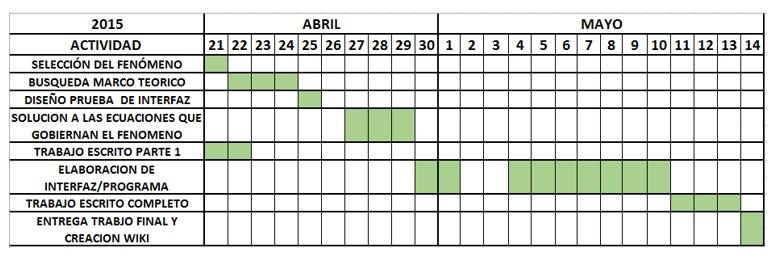
\includegraphics[width=1\textwidth]{images/agenda.jpg}
    \fontetabela{\textbf{Fonte:} Elaborado pelos autores (2026).}
\end{figure}

\section{Matriz SWOT}

A Matriz SWOT constitui uma ferramenta de apoio à análise estratégica, permitindo identificar os pontos fortes e fracos de um projeto, bem como as oportunidades e ameaças presentes no ambiente externo. Nesse sentido, a Figura \ref{fig:swot} ilustra as principais vantagens e desvantagens do produto desenvolvido.

\begin{figure}[H]
    \centering
    \caption{Matriz SWOT.}
    \label{fig:swot}
    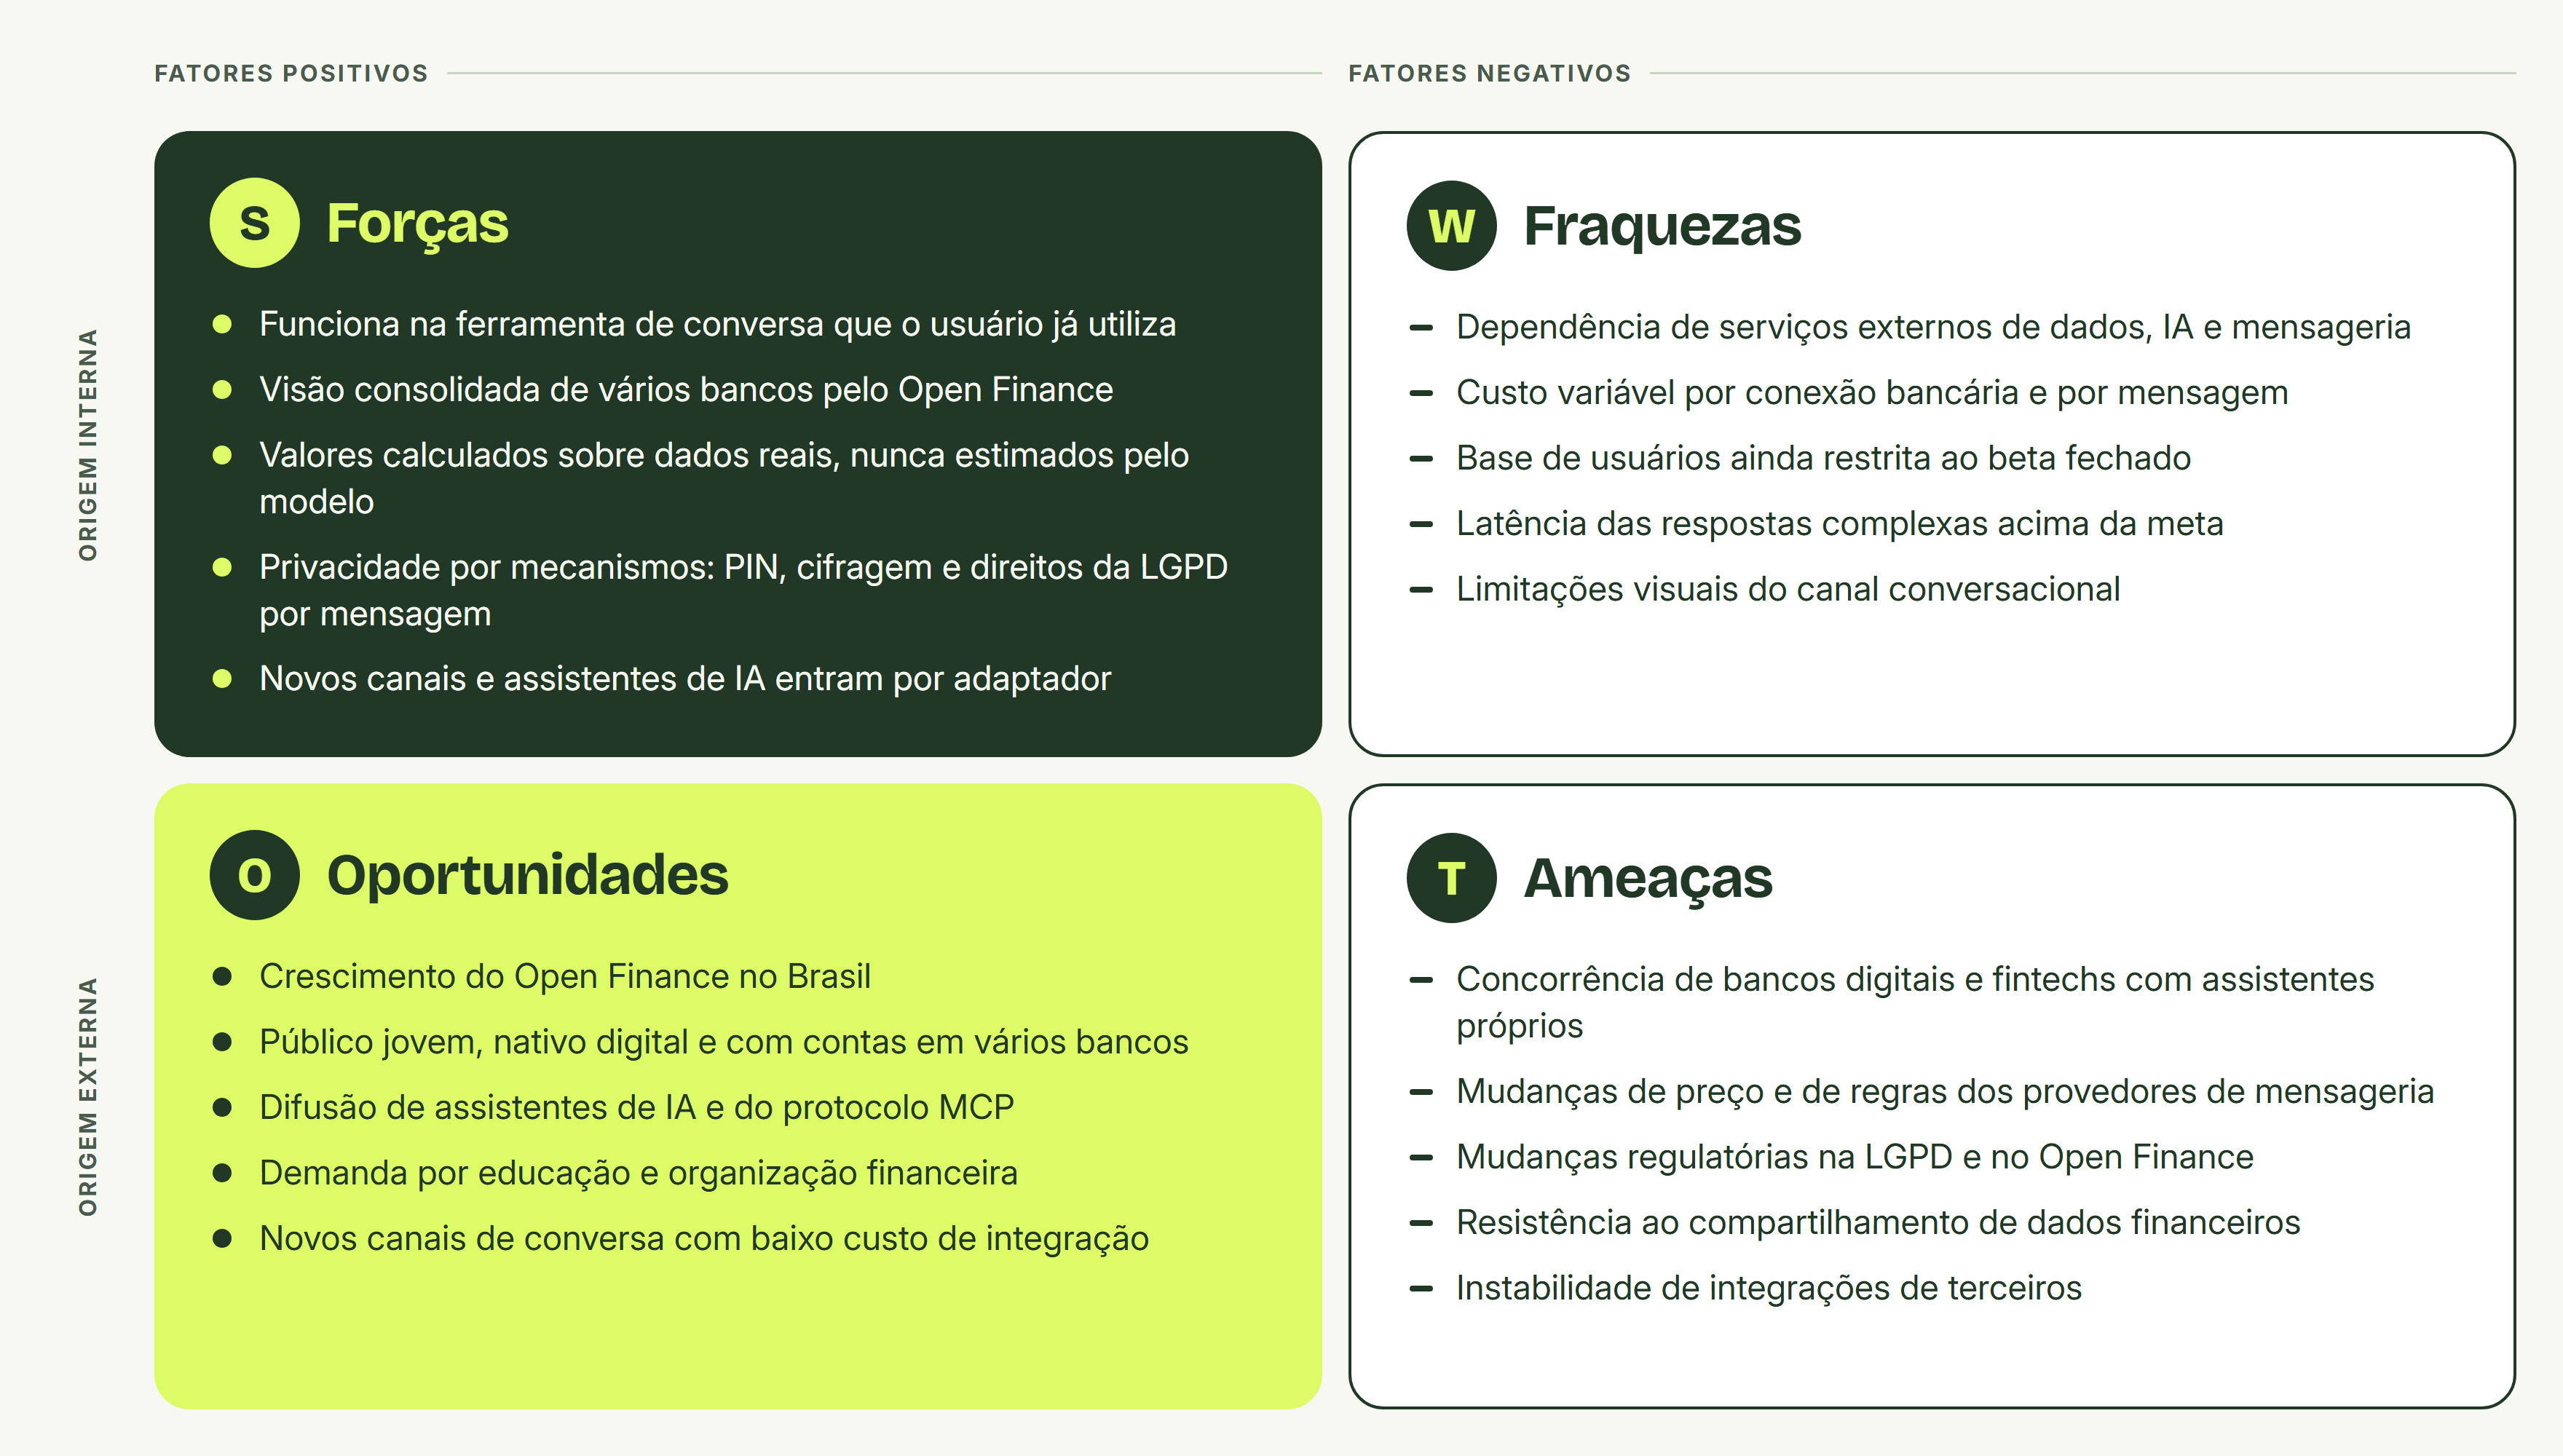
\includegraphics[width=1\textwidth]{images/swot.png}
    \fontetabela{\textbf{Fonte:} Elaborado pelos autores (2026).}
\end{figure}
